\chapter{Manufacturing of Planar Detectors}
The manufacturing process of a planar HPGe detector begins with a slice from a crystal boule that has been tested for quality and is know to be detector grade. Typical boules slices are solid discs that can range from a few millimeters up to several centimeters in thickness and 5+ centimeters in diameter. This large size allows for several detector samples to be cut from each slice so careful geometry considerations are important in order to minimize wasted material.
\begin{figure}[htpb]
\centering
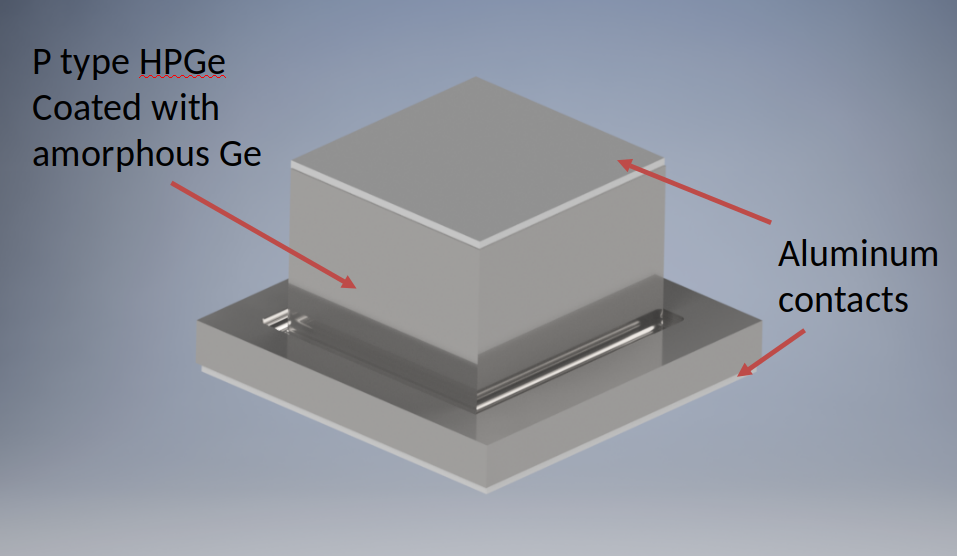
\includegraphics[width=0.5\textwidth]{dummy-det}
\caption{Example detector geometry with four wings}
\label{dummydet}
\end{figure}


\subsection{Mechanical Processing}

\begin{figure}[htpb]
\centering
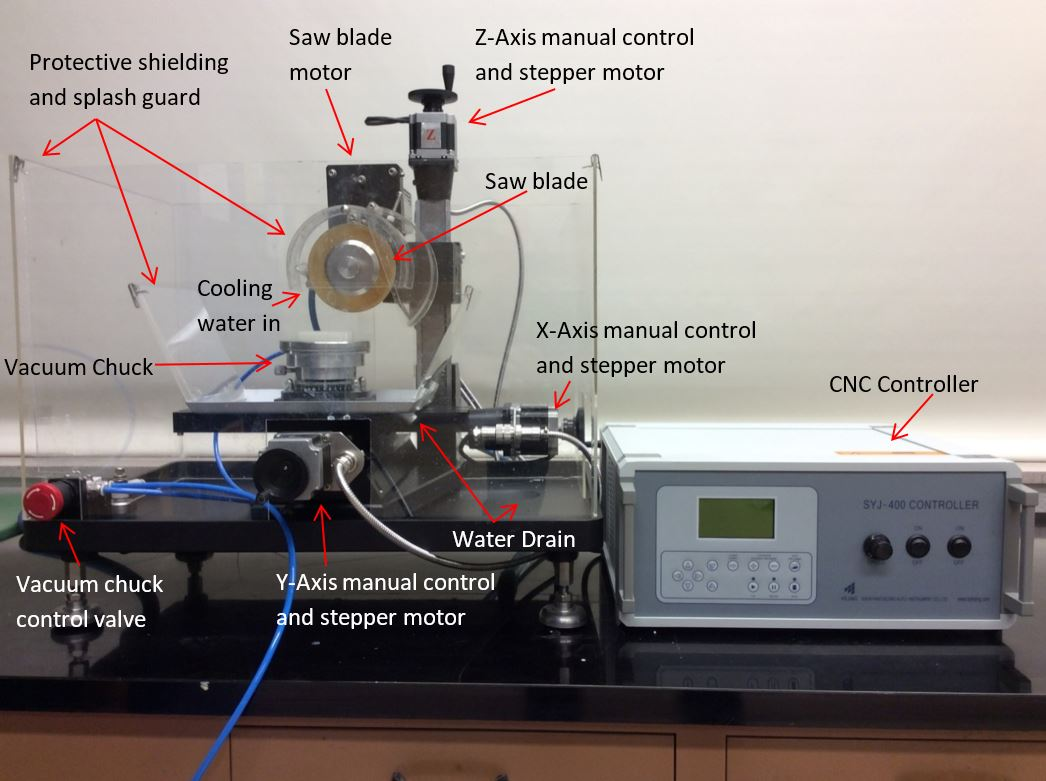
\includegraphics[width=0.5\textwidth]{diamond-saw.jpg}
\caption{The diamond saw used to cut boules into detector samples.}
\label{diamondsaw}
\end{figure}

\begin{figure}[htpb]
\centering
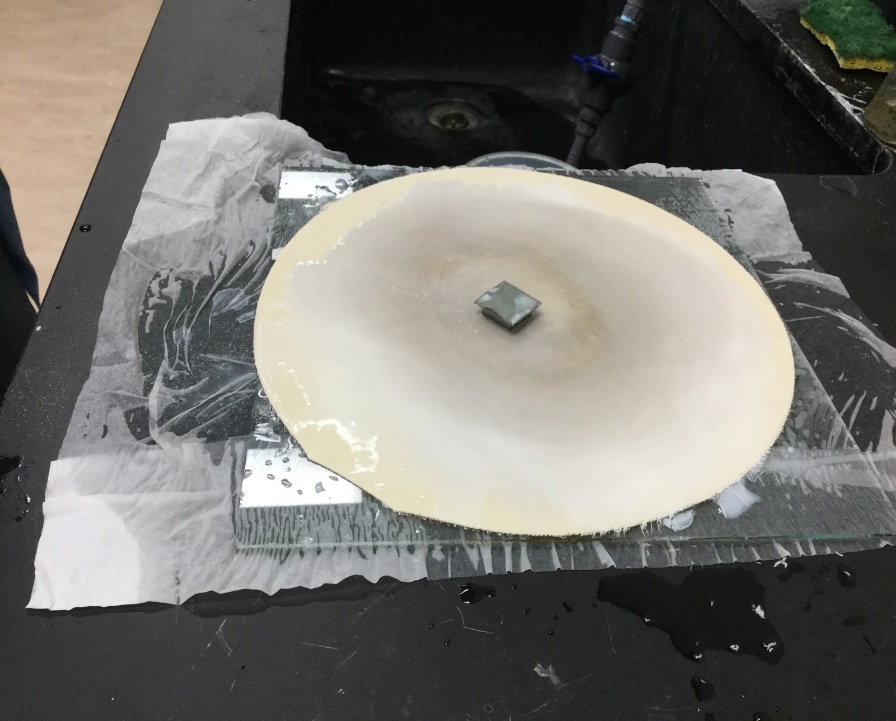
\includegraphics[width=0.5\textwidth]{lapping.jpg}
\caption{An example of lapping the detector sample}
\label{lapping}
\end{figure}

\subsection{Chemical Processing}

\begin{figure}[htpb]
\centering
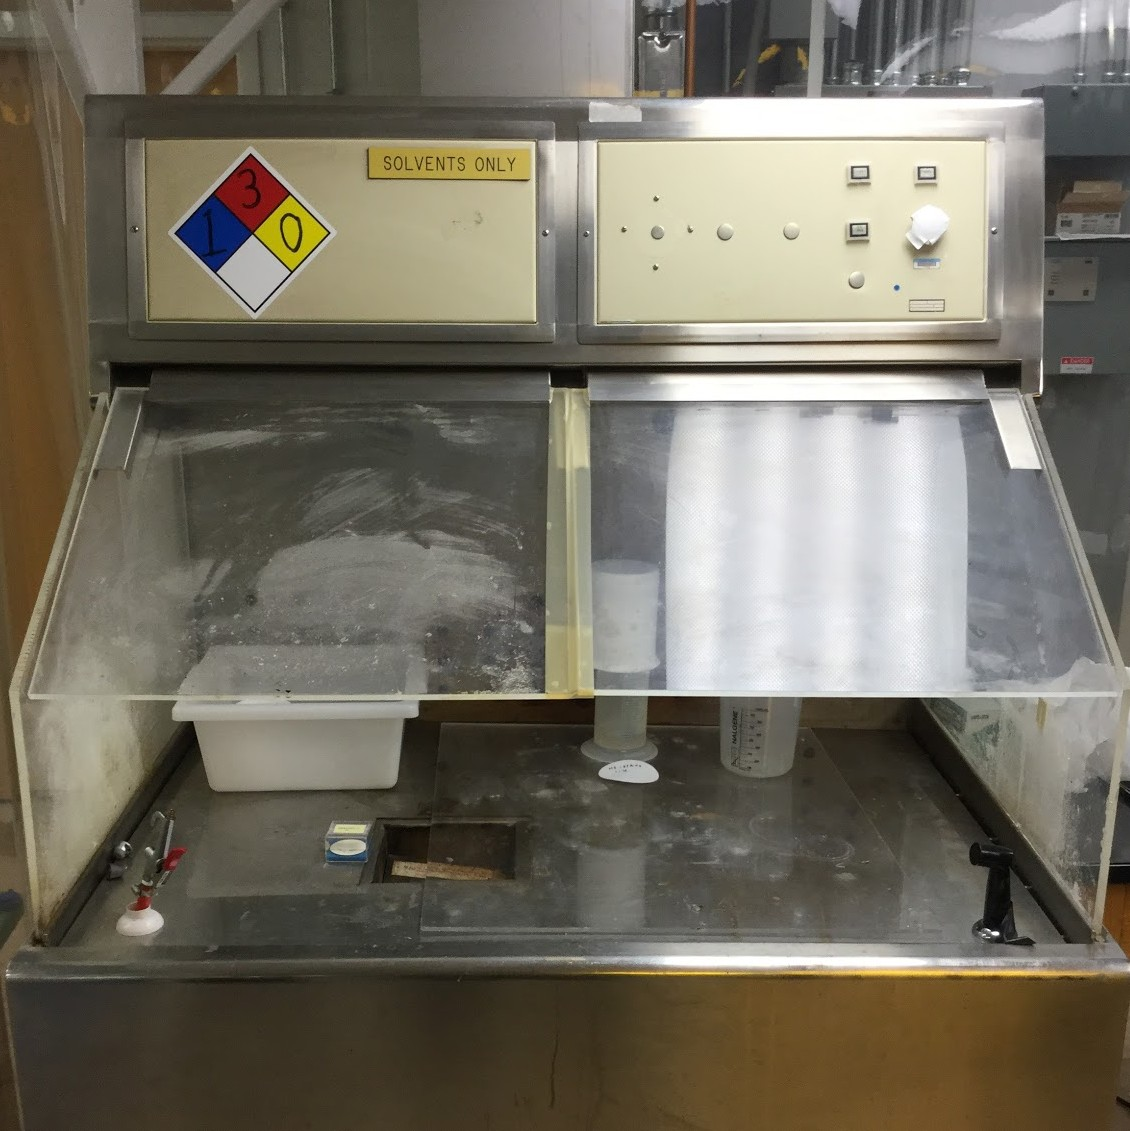
\includegraphics[width=0.5\textwidth]{metal-hood.jpg}
\caption{Metal hood for use with solvents}
\label{metalhood}
\end{figure}


\begin{figure}[htpb]
\centering
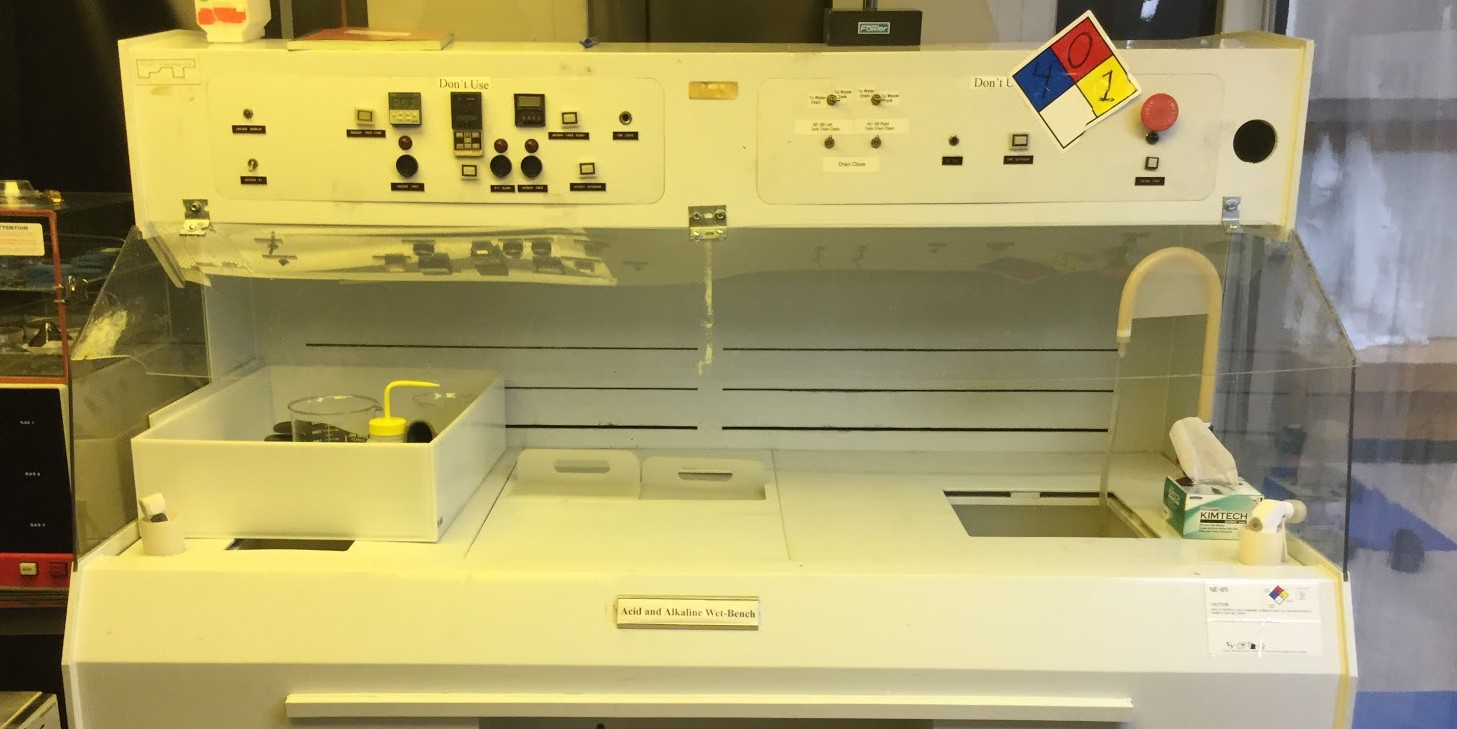
\includegraphics[width=0.5\textwidth]{plastic-hood.jpg}
\caption{Plastic hood for use with acids.}
\label{plastichood}
\end{figure}



\subsection{Amorphous Ge Deposition}

\begin{sidewaysfigure}
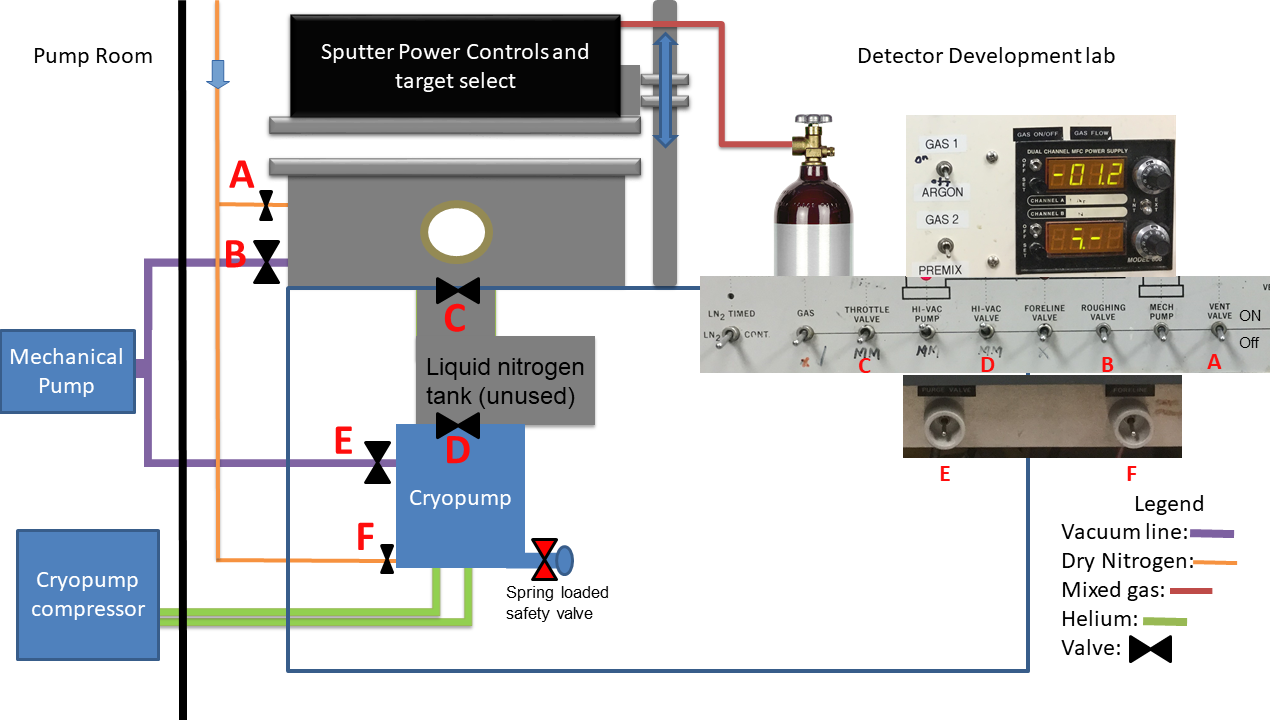
\includegraphics[width=\textwidth]{sput-flow}
\caption{This is a diagram of the Sputtering machine vacuum and gas system. Each valve is connected to a pressurized air line.}
\label{LandscapeFigure}
\end{sidewaysfigure}

\subsection{Aluminum Deposition}

\begin{sidewaysfigure}
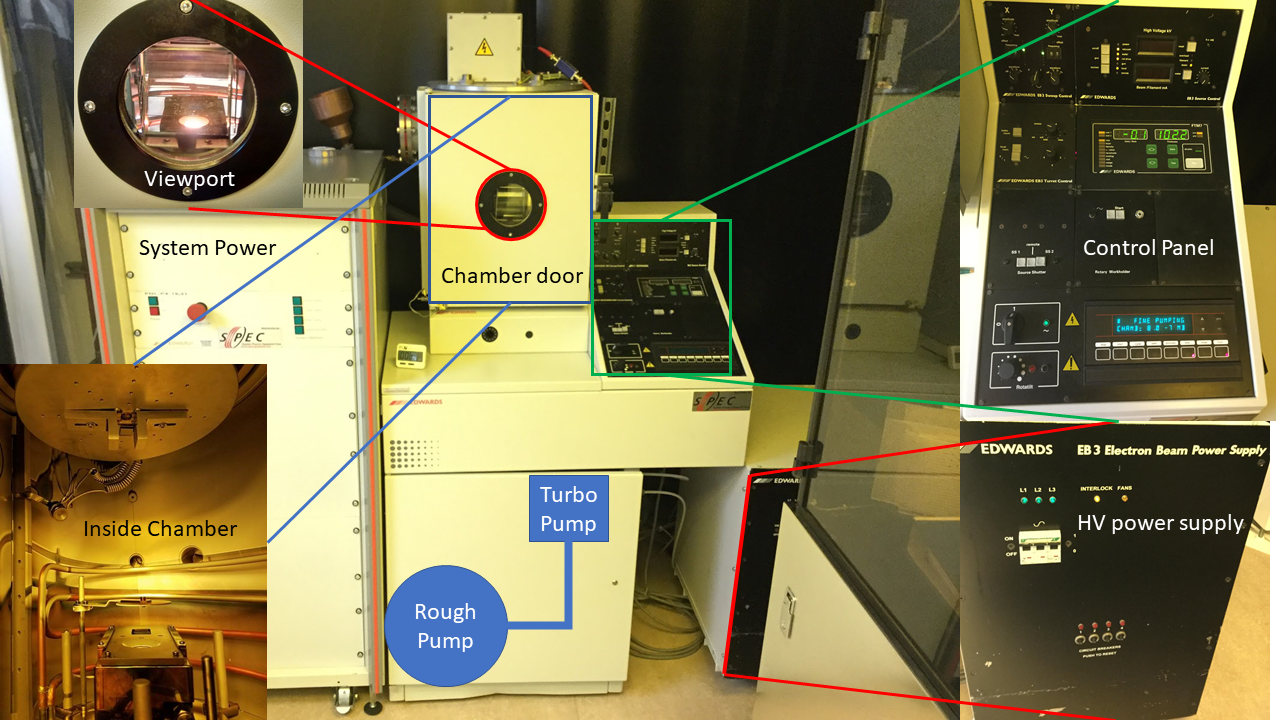
\includegraphics[width=\textwidth]{ebeam-flow}
\caption{This is a diagram of the of the electron beam machine.It is used to deposit aluminum onto the detector sample.}
\label{LandscapeFigure}
\end{sidewaysfigure}


\subsection{Final Steps}
